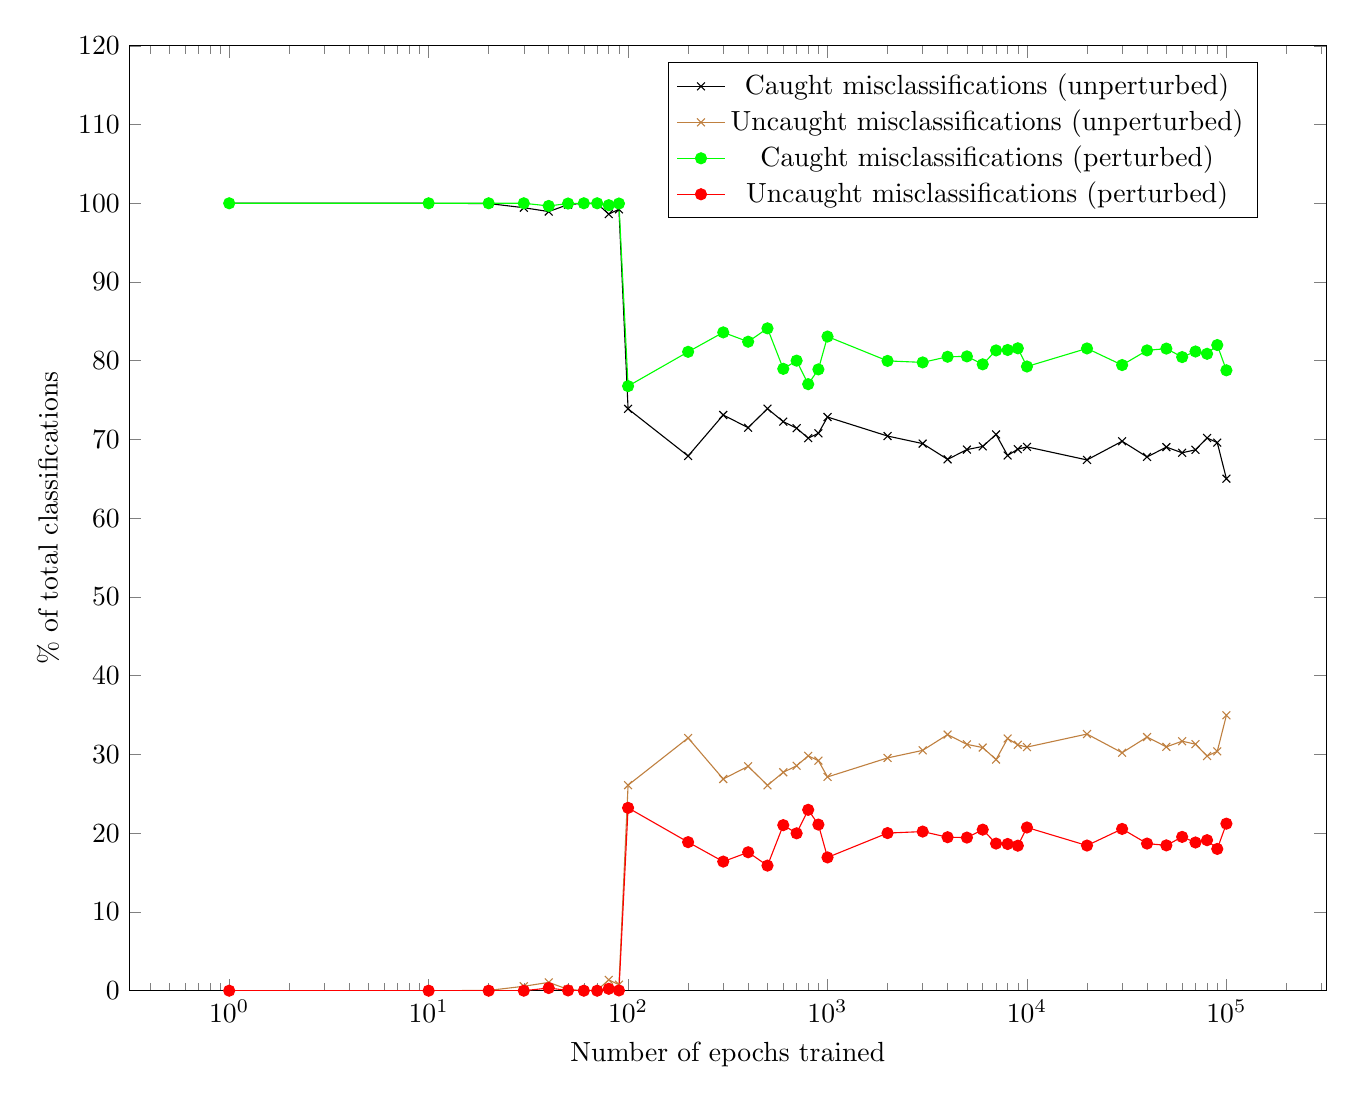
\begin{tikzpicture}
\begin{semilogxaxis}[
xlabel={Number of epochs trained},
ylabel={\% of total classifications},
x=1.1cm, y=1.0mm, 
ymin=0, ymax=120,
legend style={at={(0.45,0.9)},anchor=west}]

\addplot[color=black,mark=x] coordinates {
	(1, 100.000000)
	(10, 100.000000)
	(20, 99.968513)
	(30, 99.438622)
	(40, 98.948822)
	(50, 99.831619)
	(60, 100.000000)
	(70, 99.946243)
	(80, 98.629845)
	(90, 99.235352)
	(100, 73.896217)
	(200, 67.904327)
	(300, 73.114166)
	(400, 71.500191)
	(500, 73.917786)
	(600, 72.264412)
	(700, 71.438644)
	(800, 70.175438)
	(900, 70.787399)
	(1000, 72.854225)
	(2000, 70.439842)
	(3000, 69.480080)
	(4000, 67.477409)
	(5000, 68.717560)
	(6000, 69.121811)
	(7000, 70.645164)
	(8000, 67.972473)
	(9000, 68.772896)
	(10000, 69.063011)
	(20000, 67.405907)
	(30000, 69.780220)
	(40000, 67.787842)
	(50000, 69.032257)
	(60000, 68.315018)
	(70000, 68.693977)
	(80000, 70.194382)
	(90000, 69.604439)
	(100000, 65.025040)
};

\addplot[color=brown,mark=x] coordinates {	
	(1, 0.000000)
	(10, 0.000000)
	(20, 0.031486)
	(30, 0.561380)
	(40, 1.051184)
	(50, 0.168381)
	(60, 0.000000)
	(70, 0.053759)
	(80, 1.370155)
	(90, 0.764649)
	(100, 26.103786)
	(200, 32.095673)
	(300, 26.885832)
	(400, 28.499805)
	(500, 26.082212)
	(600, 27.735594)
	(700, 28.561354)
	(800, 29.824560)
	(900, 29.212601)
	(1000, 27.145777)
	(2000, 29.560154)
	(3000, 30.519920)
	(4000, 32.522587)
	(5000, 31.282434)
	(6000, 30.878185)
	(7000, 29.354836)
	(8000, 32.027523)
	(9000, 31.227106)
	(10000, 30.936995)
	(20000, 32.594090)
	(30000, 30.219782)
	(40000, 32.212166)
	(50000, 30.967743)
	(60000, 31.684982)
	(70000, 31.306025)
	(80000, 29.805618)
	(90000, 30.395559)
	(100000, 34.974957)
};

\addplot[color=green,mark=*] coordinates {	
	(1, 100.000000)
	(10, 100.000000)
	(20, 100.000000)
	(30, 100.000000)
	(40, 99.662552)
	(50, 99.968597)
	(60, 100.000000)
	(70, 100.000000)
	(80, 99.758133)
	(90, 99.968475)
	(100, 76.780945)
	(200, 81.134331)
	(300, 83.604851)
	(400, 82.419716)
	(500, 84.116234)
	(600, 78.973373)
	(700, 80.015221)
	(800, 77.028572)
	(900, 78.905663)
	(1000, 83.074722)
	(2000, 79.983315)
	(3000, 79.792389)
	(4000, 80.510559)
	(5000, 80.555107)
	(6000, 79.547066)
	(7000, 81.314125)
	(8000, 81.369659)
	(9000, 81.582603)
	(10000, 79.271027)
	(20000, 81.565376)
	(30000, 79.456421)
	(40000, 81.315414)
	(50000, 81.545204)
	(60000, 80.468216)
	(70000, 81.178162)
	(80000, 80.884285)
	(90000, 81.995102)
	(100000, 78.786835)
};

\addplot[color=red,mark=*] coordinates {
	(1, 0.000000)
	(10, 0.000000)
	(20, 0.000000)
	(30, 0.000000)
	(40, 0.337446)
	(50, 0.031402)
	(60, 0.000000)
	(70, 0.000000)
	(80, 0.241872)
	(90, 0.031525)
	(100, 23.219051)
	(200, 18.865665)
	(300, 16.395145)
	(400, 17.580284)
	(500, 15.883766)
	(600, 21.026627)
	(700, 19.984774)
	(800, 22.971428)
	(900, 21.094332)
	(1000, 16.925280)
	(2000, 20.016680)
	(3000, 20.207613)
	(4000, 19.489441)
	(5000, 19.444899)
	(6000, 20.452932)
	(7000, 18.685873)
	(8000, 18.630341)
	(9000, 18.417391)
	(10000, 20.728970)
	(20000, 18.434624)
	(30000, 20.543579)
	(40000, 18.684584)
	(50000, 18.454794)
	(60000, 19.531784)
	(70000, 18.821840)
	(80000, 19.115713)
	(90000, 18.004898)
	(100000, 21.213161)
};

\legend{Caught misclassifications (unperturbed), Uncaught misclassifications (unperturbed), Caught misclassifications (perturbed), Uncaught misclassifications (perturbed)}
\end{semilogxaxis}%
\end{tikzpicture}%